% !TeX root = ../main.tex
% Add the above to each chapter to make compiling the PDF easier in some editors.

\chapter{Design and Implementation}\label{chapter:design_and_implementation}
This chapters explains the design and implementation details. All of the sections in this chapter are divided into Concepts, Implementation and Configuration subsections.
\section{Maps}
This section explains how maps are used, and how to prepare and configure maps for ONE simulator.
	\subsection{Concept}
	Maps play a very important role in simulating real-world depiction of any place in the ONE simulator. This allows us to simulate the physical location as accurately as possible. The \textit{MapBased Movement} provides us with different types of map-related movements.

	The ONE Simulator requires the map in the modified Well-Known Text (WKT) Format. I call it the modified version as the WKT files utilizes points based system instead of coordinates based system. We use the Osm2Wkt tool\cite{mayer2010osm} for converting Open Street Maps (OSM) files to WKT for the ONE Simulator.

	\subsubsection {Filtering Maps}
	The ONE Simulator can accept one or more WKT map files. In case of more than 1 files, all of the files are basically overlayed on the top of each other. One thing to note is that the files need to be fully connected otherwise the ONE simulator won't start and will throw an error.

	OpenStreetMap provides with a tool called OSMFilter \cite{osm-filter} which enables us to filter the OSM maps. This allows us to filter specific elements such as roads, bus routes etc. To use the filtered maps with ONE simulator, we need to convert each of them to WKT.
	The current implementation of the ONE simulator uses the following 4 WKT files:

	\begin{center}
    	\captionof{table}{ONE Simulator: WKT Map files used by default} \label{tab:wktMapFiles}
	    \begin{tabular}{ | l | p{10.5cm} |}
    		\hline
    		\textbf{Map File} & \textbf{Details} \\ \hline
    		\textit{main\_roads.wkt} & represents the main roads (primary, secondary, tertiary). \\ \hline
    		\textit{roads.wkt} & represents the normal roads and streets.  \\ \hline
    		\textit{shops.wkt} & represents the shops. \\ \hline
    		\textit{pedestrian\_paths.wkt} & represents the pedestrian paths. \\ \hline
    	\end{tabular}
	\end{center}

	\subsubsection{OSM Maps}
	The first step in getting the maps is to download the OSM map from the Open Street Map export tool \cite{openstreetmap-export}. Figure~\ref{fig:munich-map} shows the OSM Map for Central Munich.
	\newline
	\begin{figure}[h]
		\centering
		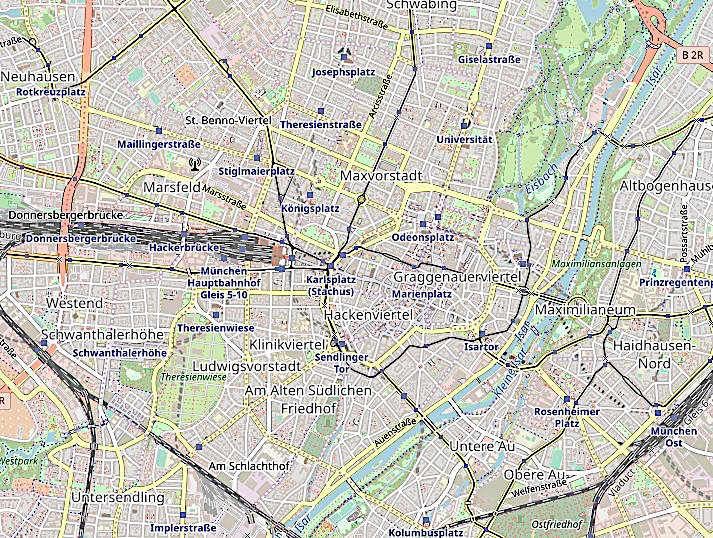
\includegraphics[scale=0.5]{./figures/central-munich-osm}
		\caption{Central Munich OSM Map - from OpenStreetMaps \cite{openstreetmap}}
		\label{fig:munich-map}
	\end{figure}

	\subsubsection{Conversion to WKT}
	There are a number of tools that can convert an OSM to WKT, however, there are a few reasons we do not use any of those tools:
	\begin{itemize}
 	 \item These tools just perform the conversion (but do not make sure the converted maps are fully connected).
   	 \item These tools do not convert the coordinates to the points-based system (which is used by the ONE simulator). To use any WKT file with the ONE simulator, we need to do proper coordinates conversion.
	\end{itemize}
	\vspace{3mm}
	Figure~\ref{fig:wkt-file} shows the contents of the WKT file. This file is generated using OpenJump \cite{openjump}, so they are in the normal coordinates system. In other words, these files are not in the coordinates system used by ONE simulator.
	\vspace{2mm}
	\begin{figure}[H]
		\centering
		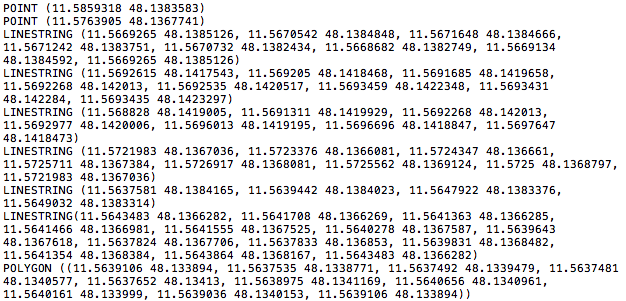
\includegraphics[scale=0.45]{./figures/wkt-file-2}
		\caption{Snapshot of WKT File Contents - Converted using OpenJump \cite{openjump} }
		\label{fig:wkt-file}
	\end{figure}
	Using OSM2WKT tool \cite{mayer2010osm}, we can convert the OSM file to a fully-connected point-based WKT file that can be used with the ONE Simulator. Figure~\ref{fig:wkt-file-for-one} shows the contents of such a WKT file.
	\vspace{2mm}
	\begin{figure}[H]
		\centering
		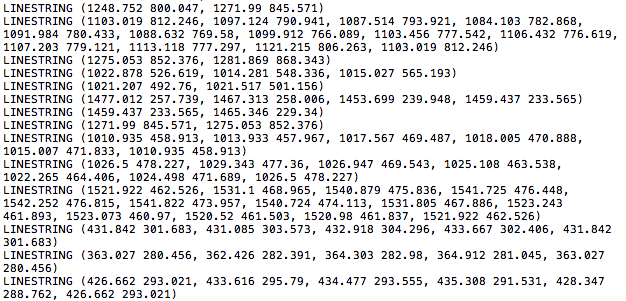
\includegraphics[scale=0.45]{./figures/wkt-file-1}
		\caption{Snapshot of WKT File Contents - Converted using OSM2WKT tool \cite{mayer2010osm} }
		\label{fig:wkt-file-for-one}
	\end{figure}
	\newpage
	Figure~\ref{fig:central-munich-wkt} shows a fully connected WKT map of central Munich.
	\vspace{6mm}
	\begin{figure}[H]
		\centering
		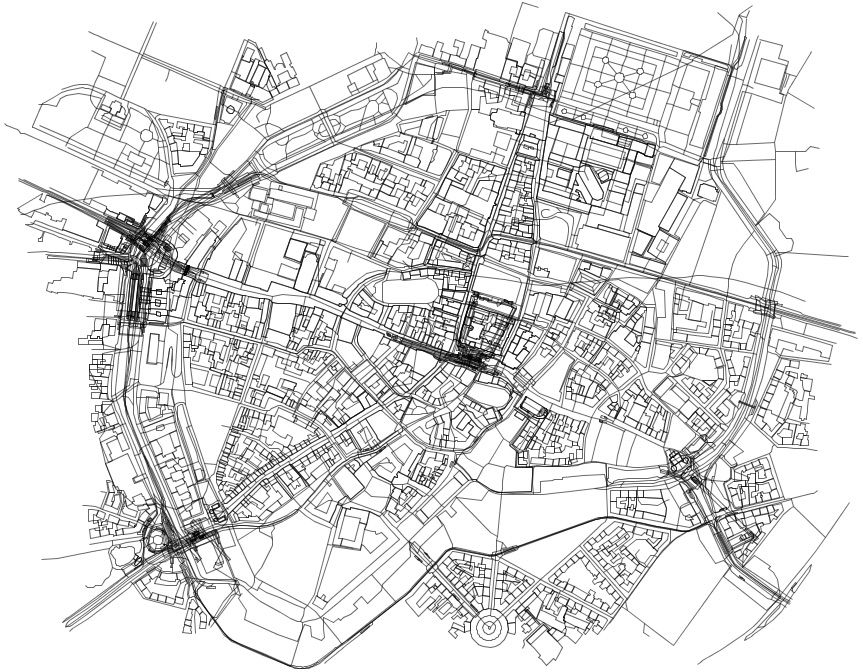
\includegraphics[scale=0.5]{./figures/central-munich-wkt}
		\caption{Central Munich WKT Map - Created using OSM2WKT tool \cite{mayer2010osm} and Screenshot using OpenJump \cite{openjump}}
		\label{fig:central-munich-wkt}
	\end{figure}
	\vspace{3mm}
We use the above map (Figure~\ref{fig:central-munich-wkt}) in our simulations. This map works fine with ONE simulator as it is a fully connected map and it has also been converted to the points-based system used by ONE simulator.
\newpage
\subsection{Implementation}
This section list and explains all the steps needed to configure and run a new map (downloaded from OpenStreetMap \cite{openstreetmap}) in ONE simulator.
\subsubsection{OSM to WKT}
Using OSM2WKT tool \cite{mayer2010osm}, any OSM file can be converted into a fully connected WKT file for use in the ONE simulator. Below are the details of how to use the OSM2WKT tool \cite{mayer2010osm} to generate a WKT file:\newline

\begin{lstlisting}[language=bash]
java -jar ./osm2wkt.jar mapfile.osm

options:
	-o outputfile - specifying the output file. In case no outputfile is mentioned, .wkt is appended to the name of input file.
	-a - open the output file in append mode (adding the wkt output at the end of the output file)
	-t deltaX deltaY - translate map by deltaX and deltaY meters
\end{lstlisting}
\captionof{lstlisting}{Using OSM2WKT tool \cite{mayer2010osm} to generate WKT}

\vspace{8mm}
The OSM2WKT tool \cite{mayer2010osm} performs a number of operations on the OSM file. It loads the map from the OSM file. The coordinates are converted to the points based system where:
   	 	\begin{enumerate}
	   	 	\item The bounding box of the map is converted into a point based system (width and height in meters).
   		 	\item All the coordinates are converted to the point based system.
   		 \end{enumerate}
   	 The completeness of the graph is then checked and all the unconnected edges are deleted so that we have a complete graph. At this stage, the file can be saved to disk as a WKT fie.

\subsubsection{Filtering OSM}
In order to filter OSM files, OSM Filter tool \cite{osm-filter} is needed. Here is the basic syntax to use the OSM Filter tool.  \cite{osm-filter}. This tool has a number of folders that we can use. Below is the common ones (for our scenario):

\begin{enumerate}
	\item  \textbf{highway}: highway represents any route/path such as roads, cycle paths, pedestian paths etc. Some examples of highway include primary, secondary, trunk, residential, service, footway, pedestrian etc.
	\item \textbf{shop}: shop represents any type of shop.

\end{enumerate}
\vspace{2mm}
\begin{lstlisting}[language=bash]
	osmfilter inputfile.osm --keep="{condition}" > outputfile.osm
\end{lstlisting}
\captionof{lstlisting}{How to use the OSM Filter tool \cite{osm-filter}}
\vspace{5mm}

The listings below show how to create the four different types of OSM files which can then be converted to WKT files.
\vspace{5mm}
\begin{lstlisting}[language=bash]
// Filtering primary, secondary, tertiary (*ary), and trunk roads as main roads.
osmfilter mapfile.osm --keep="highway=*ary trunk" > main_roads.osm

// Filtering residential roads, living street (street with special rules), service and link roads as the common roads
osmfilter mapfile.osm --keep="highway=residential service *link living_street" > roads.osm

// Filtering pedestrian footway living_street as pedestrian paths.
osmfilter map.osm --keep="highway=pedestrian footway living_street" > pedestrian_paths.osm

// Filtering all shops as shops.
osmfilter map.osm --keep="shop=*" > shops.osm
\end{lstlisting}
\captionof{lstlisting}{Filtering OSM files}
\vspace{5mm}

The main issue with using separate osm files is that we cannot use Osm2WKT tool \cite{mayer2010osm} and it is a difficult task to make sure the resultant map is fully connected. The Osm2WKT tool \cite{mayer2010osm} can be modified to accept more than 1 OSM files and generate the corresponding WKT files that are fully connected. The main idea is to read all of the OSM files and place them on one graph. Now we start dropping unconnected nodes and paths until we have a fully connected map that can be used by ONE simulator. We are using a single map file in our simulations.

\subsection{Configuration}
In order to utilize the \textit{MapBasedMovement} and the map files we have prepared (using method in the above sections), We need to add a few things to the configuration file.

\begin{enumerate}
	\item The first step is to set the \textit{movementModel} of the desired group to \textit{MapMapMovement}. This tells the ONE simulator to use map-based movement for these groups.
	\begin{lstlisting}[language=bash]
	Group.movementModel = MapBasedMovement
	\end{lstlisting}
	\item Then we need to identify the number of maps files we are providing and provide the relative path to each of the maps files.
	\begin{lstlisting}[language=bash]
	MapBasedMovement.nrofMapFiles = 1
	MapBasedMovement.mapFile1 = data/maps/map.wkt
	\end{lstlisting}
\end{enumerate}

We can also add more than one map files. Below is an example of using more than 1 map files.

\begin{lstlisting}[language=bash]
MapBasedMovement.nrofMapFiles = 4

MapBasedMovement.mapFile1 = data/maps/roads.wkt
MapBasedMovement.mapFile2 = data/maps/main_roads.wkt
MapBasedMovement.mapFile3 = data/maps/pedestrian_paths.wkt
MapBasedMovement.mapFile4 = data/maps/shops.wkt

\end{lstlisting}

In this section, we have discussed how to prepare map files for the ONE simulator and how to configure the ONE simulator to use those files.

\section{Access Points}
In this section, we will introduce the concept of access points and how they are implemented in the ONE simulator.
\subsection{Concept}
Access Points are devices that connect devices to one another and facilities the flow of information among devices. One of an interesting use case would be to connect the nodes to the internet using these access points. An Access Point can operate in any of the following three modes:

	\begin{center}
    	\captionof{table}{ONE Simulator: Modes of Operation for Access Points/Wifi Interface}
	    \begin{tabular}{ | l | p{10.5cm} |}
    		\hline
    		\textbf{Mode} & \textbf{Description} \\ \hline
    		\textit{Access Point (AP)} & Access Point (AP) provides a bridge for two Station Adapters (SAs) to connect and communicate with each other. Two Access Points cannot talk to each other directly. \\ \hline
    		\textit{Station Adapter (SA)} & Station Adapter (SA) is a passive device that can connect to an Access Point and communicate to other Station Adapters using the Access Point (AP). Two Station Adapters cannot talk to each other directly. \\ \hline
    		\textit{Ad-hoc} & Ad-hoc Mode is used when we want two devices to connect and communicate directly to each other. Hosts in Ad-hoc mode cannot connect to either an Access Point (AP) or Station Adapter(SA) and vice versa. This is the default mode.\\ \hline
    	\end{tabular}
	\end{center}
	\vspace{5mm}
	Figure~\ref{fig:aps1} shows the color scheme used by ONE simulator to differentiate between nodes with different modes of operation. It also differentiates between normal and access point enabled hosts.\newline
	\begin{figure}[h]
		\centering
		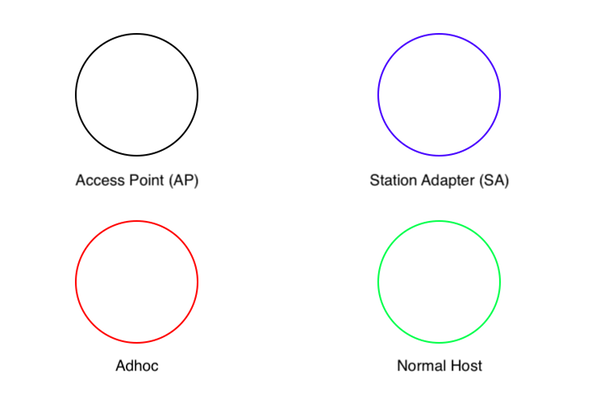
\includegraphics[scale=0.45]{./figures/aps-1}
		\caption{Hosts with Access Points (SA, AP, and Ad-hoc) and Normal Host}
		\label{fig:aps1}
	\end{figure}
	\newpage
	Below is a screenshot from the ONE Simulator with all of the above hosts in action.\newline
	\begin{figure}[H]
		\centering
		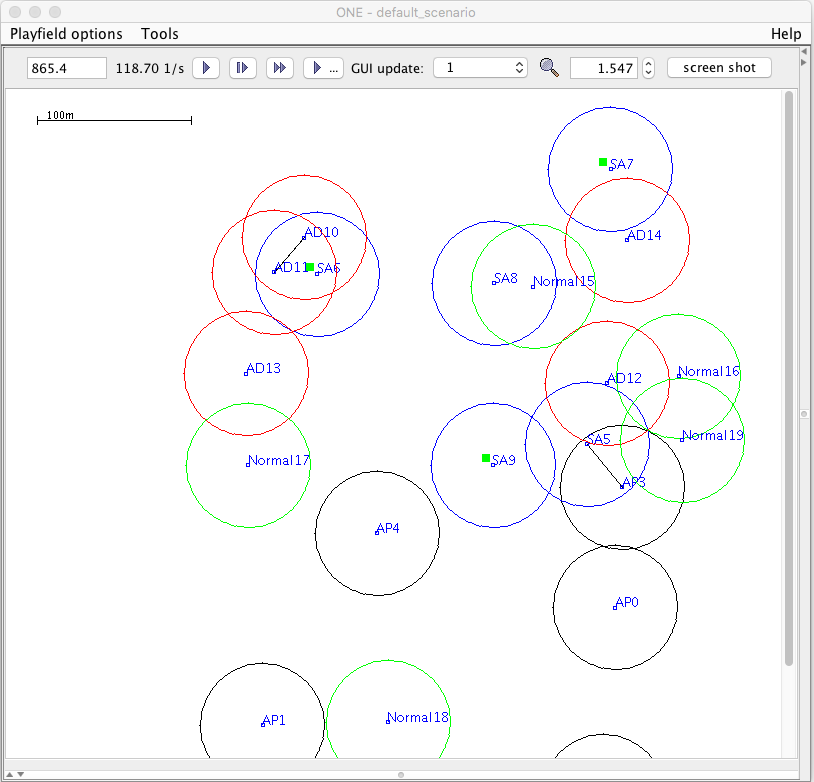
\includegraphics[scale=0.5]{./figures/aps-2}
		\caption{ONE Simulator showing all the Hosts (AP enabled and normal) in action}
	\end{figure}
	The above figure shows that station adapters can connect to an access point (\textit{SA5} and \textit{AP3}), ad-hoc nodes can connect to other ad-hoc nodes (\textit{AD10} and \textit{AD11}), ad-hoc nodes cannot connect to access points and vice versa (\textit{AD10}), \textit{AD11} and \textit{SA6}). It also shows that the normal hosts cannot connect to access points enabled hosts (\textit{Normal15} and \textit{SA8}, \textit{Normal16} and \textit{AD12} etc.).

\newpage
\subsection{Implementation}
Before discussing implementation details, We would like to discuss the pre-requisite for the implementation. The following table lists two classes and what they are used for:
	\begin{center}
	    \begin{tabular}{ | l | p{10.5cm} |}
    		\hline
    		\textbf{Class} & \textbf{Description} \\ \hline
    		\textit{DTNHost} & This class represents a DTN Capable host. It contains all the properties and functionalities for the host such as groupID, MessageListeners, MovementListeners etc. \\ \hline
    		\textit{DTNHostWithWifi} & This class is a subclass of the \textit{DTNHost} class and represents a host with Access Point/Wifi capability. It inherits everything from the parent class and adds an extra mode (which can either be ADHOC, AP or SA). \\ \hline
    	\end{tabular}
       	\captionof{table}{ONE Simulator: Classes related to Hosts/Nodes}
	\end{center}
\vspace{5mm}
\textit{DTNHostWithWifi} is a very lean host that takes everything from its parent \textit{DTNHost} and adds the mode. The following listing shows the implementation of \textit{DTNHostWithWifi}.\newline
\begin{lstlisting}[language=java]
public class DTNHostWithWifi extends DTNHost {
	public static int AP = 1;
	public static int SA = 2;
	public static int ADHOC = 3;
	private int mode;

	public DTNHostWithWifi(other parameters, String mode) {
	 ...
	 this.mode = mode.equalsIgnoreCase("ap") ? AP : mode.equalsIgnoreCase("sa") ? SA : ADHOC;
	}

	public int getMode() {
		return mode;
	}
}
\end{lstlisting}
\captionof{lstlisting}{ONE Simulator: DTNHostWithWifi Implementation}
\label{listing:dtnhostwithwifi}
\vspace{4mm}
In Listing~\ref{listing:dtnhostwithwifi}, \textit{DtnHostWithWifi(..)} initializes the mode with the passed value. It also sets the default mode of operation to ad-hoc (in case an empty or wrong mode is specified). \textit{getMode} returns the mode of operation.\newline
\newline
There is another component that needs to be implemented i.e. an interface to the new \textit{DTNHostWithWifi}. We call it \textit{WifiInterface}. The following table discusses the two main classes.

\begin{center}
    	\captionof{table}{ONE Simulator: WifiInterface \& its parent interface}
	    \begin{tabular}{ | l | p{10cm} |}
    		\hline
    		\textbf{Class} & \textbf{Description} \\ \hline
    		\textit{SimpleBroadcastInterface} & \textit{SimpleBroadcastInterface} is a Network Interface that is responsible for connectivity among hosts. It allows one-to-one transmission with a constant bit-rate.\\ \hline
    		\textit{WifiInterface} & \textit{WifiInterface} is responsible for connectivity between two different \textit{DTNHostWithWifi} objects. It is also responsible that the connection rules (SA can connect only to AP, Ad-hoc hosts can connect to each other only) are upheld. \\ \hline
    	\end{tabular}
	\end{center}
\vspace{3mm}
\textit{WifiInterface} takes almost everything from its parent but adds the extra ability to check if two \textit{DTNHostWithWifi} can connect to each other. Another method that it overrides is the ability to return \textit{DTNHostWithWifi} with the \textit{getHost()} method.\newline
\newline
Listing~\ref{listing:dtnhostwithwifi} shows a snapshot of relevant parts of \textit{WifiInterface} implementation. For the sake of simplicity, we have divided the code into numbered sections, each of which is explained below:
\begin{enumerate}
	\item \textit{connect(..)} is used to connect two hosts with wifi interfaces. It uses \textit{canConnectTo(..)} to determine if the two hosts can connect to each other. In case \textit{canConnect(..)} return true, then the transmission speed of the connection is set, which is the minimum speed of both the interfaces. The hosts are connected to each other using their interfaces.
	\item \textit{canConnectTo(..)} determines if two hosts with wifi interface connect to each other. The connectivity is based on the mode of the device. Below are the rules used to determine if two such hosts can connect to each other:
		\begin{itemize}
			\item Ad-hoc hosts (ADHOC) can connect to other ad-hoc hosts but they cannot connect to either station adapters (SA) or access points (AP).
			\item Station adapters (SA) can only connect to access points (AP) and vice versa.
		\end{itemize}
\end{enumerate}

\newpage
\begin{lstlisting}[language=java]
public class WifiInterface extends SimpleBroadcastInterface {
    //1
    public void connect(NetworkInterface anotherInterface) {
         if (canConnectTo(anotherInterface)) {
               int conSpeed = anotherInterface.getTransmitSpeed();
               if (conSpeed > this.transmitSpeed) {
                     conSpeed = this.transmitSpeed;
               }
              //Connectivity code
	        }
     }

    //2
     boolean canConnectTo(NetworkInterface anotherInterface) {
          ...
          if(canConnect) {
                WifiInterface thisInterface = (WifiInterface) this;
                WifiInterface secondInterface = (WifiInterface) anotherInterface;

                int thisInterfaceMode = thisInterface.getHost().getMode();
                int secondInterfaceMode = secondInterface.getHost().getMode();

                if(thisInterfaceMode == DTNHostWithWifi.ADHOC) {
                      canConnect = thisInterfaceMode == secondInterfaceMode;
                } else {
                      canConnect = (thisInterfaceMode == DTNHostWithWifi.AP && secondInterfaceMode == DTNHostWithWifi.SA) || (thisInterfaceMode == DTNHostWithWifi.SA && secondInterfaceMode == DTNHostWithWifi.AP);
                }
           }
           return canConnect;
      }
      ...
}
\end{lstlisting}
\captionof{lstlisting}{ONE Simulator: WifiInterface Implementation}
\label{listing:dtnhostwithwifi}
\newpage

Now, we need to combine both of these to make sure that any host having a \textit{WifiInterface} is instantiated as \textit{DTNHostWithWifi} objects and all the other hosts are instantiated as \textit{DTNHost} objects. This needs to be done inside \textit{createHosts()} function of \textit{SimScenario} class. Below are the changes that are made to achieve this purpose:
\vspace{3mm}
\begin{lstlisting}[language=java]
			boolean hasWifiInterface = false;

			//1.
			for (int j=1;j<=nrofInterfaces;j++) {
				...
				if(iface instanceof WifiInterface) {
					hasWifiInterface = true;
				}
				...
			}
			...
			//2.
			List<String> modes = new ArrayList<String>();
			String wifiMode = s.getSetting("mode",null);

			if(wifiMode == null) {
				String modesFile = s.getSetting("modesFile",null);
				if(modesFile != null) {
					try {
						Scanner in = new Scanner(new FileReader(modesFile));
						while(in.hasNextLine()) {
							modes.add(in.nextLine());
						}
						in.close();
					} catch (FileNotFoundException e) {}
				}
			}

			// 3.
			for (int j=0; j<nrofHosts; j++) {
				...
				if(!hasWifiInterface) {
					DTNHost host = new DTNHost(this.messageListeners,
						this.movementListeners,	gid, interfaces, comBus,
						mmProto, mRouterProto);
					hosts.add(host);
				} else {
					String mode = wifiMode != null ? wifiMode : (j < modes.size() ? modes.get(j) : "");

					DTNHostWithWifi host = new DTNHostWithWifi(this.messageListeners, this.movementListeners, gid, interfaces, comBus, mmProto, mRouterProto,  mode: mode);
					hosts.add(host);
				}
			}
		}
	}
\end{lstlisting}
\captionof{lstlisting}{ONE Simulator: Changes to SimScenario for Implementation of the AP-capable hosts}
\vspace{3mm}
The above listing performs a few operations, which are divided into the following three groups:
\begin{enumerate}
	\item In this section, we iterate through all the interfaces looking for a wifi interface (to determine if the host has access point support).
	\item In this section, we read the mode variable or the modeFile and store all of the modes.
	\item This is the section where we differentiate between normal and access points enabled hosts. This section first checks what type of host to create and in case of an access point enabled host, it sets the mode by fetching it from either the \textit{wifiMode} variable or the \textit{modes} array.
\end{enumerate}
\subsection{Configuration}
The following listing shows how to configure \textit{DTNHost} and \textit{DTNHostWithWifi}. It also shows how to configure \textit{mode} for \textit{DTNHostWithWifi} using the two different methods.

\begin{lstlisting}[language=bash]
//1.
wifiInterface.type = WifiInterface
wifiInterface.transmitSpeed = 50k
wifiInterface.transmitRange = 40

btInterface.type = SimpleBroadcastInterface
btInterface.transmitSpeed = 250k
btInterface.transmitRange = 10

//2.
Scenario.nrofHostGroups = 5

Group.nrofInterfaces = 1
Group.interface1 = btInterface

//3.
Group1.groupID = Normal

//4.
Group2.groupID = SA
Group2.interface1 = wifiInterface
Group2.mode = sa

Group3.groupID = AP
Group3.interface1 = wifiInterface
Group3.mode = ap

Group4.groupID = ADHOC
Group4.interface1 = wifiInterface
Group4.mode = ad-hoc

//5.
Group5.groupID = D
Group5.interface1 = wifiInterface
Group5.modesFile = data/modes.txt
\end{lstlisting}
Below is a summary of the above listing:
\begin{enumerate}
	\item We define two interfaces with transmission range and speed. One of the interfaces is a \textit{WifiInterface}.
	\item We are defining the general settings for the simulation and all the groups. We are setting the total number of groups to 5, the number of interfaces for each group to 1 and setting \textit{btInterface} as the default group of each group.
	\item We are setting the ID for Group1 which is using the default interface.
	\item We are defining three groups to use \textit{wifiInterface}. We are also setting the mode for each group (all the hosts of that group share the same mode)/
	\item We are defining one more group to use \textit{wifiInterface}. However, here we are setting the modes using a text file.
\end{enumerate}
\section{Snapping to Access Points}
In this section, we define a new concept known as snapping to access points.
\subsection{Concept}
Section~\ref{section:floating-content} discusses that a message is tagged with geographical coordinates and an availability/radius. \textit{Snapping to Access Point} is the concept of increasing the availability of the message beyond its original availability zone. In the configuration, we can define how many Access Points should the message snap to at maximum. Theoretically, the number of snapped Access Points should directly influence the TTL (Time to live) of the message. Below is a step-wise explanation of the process:

	\begin{enumerate}
 	 \item The host Station Adapter (\textit{SA1}) generates a message \textit{M} with a center of the anchor zone \textit{C} (which is the location of \textit{SA1} at that time), availability \textit{a} and number of maximum access points to snap to (\textit{k}). Let's assume k to be 3 \textit{k = 3}.
 	 \item \textit{SA1} comes in contact with an Access Point (\textit{AP1}), a connection is made and a copy of the message \textit{M} is transferred (\textit{M'}).
 	 \item If \textit{k}-value for the original message \textit{M} is greater than 0:
 	 	\begin{enumerate}
 	 		\item \textit{k}-value for the original message (\textit{M}) is decreased by 1.
 	 		\item \textit{k}-value for the copied message (\textit{M'}) is set to zero.
 	 		\item The center of the copied message (\textit{M'}) is changed to the center of the Access Point (\textit{AP1}).
 	 	\end{enumerate}
 	 \item The above process continues for the original message \textit{M} until \textit{k}=0.
 	 \end{enumerate}

 	Since the ID of the message \textit{M} and all of the copies is the same, they are treated as the same message; which allows us to extend the availability of the message. There are a few important points to note:
	\begin{enumerate}
 	 \item Copies of the message are not snapped to any access point, Only the original message is snapped.
 	 \item If a message is snapped to 1 access point which drops it due to any reason (apart from TTL expiry), whenever that message (the original or even the copy which knows about this access point) is copied again, it is snapped to that access point again.
 	 \item The availability zones of the copies might or might not intersect each other, however, the availability zone of the original message and each copy would have an overlap.
 	 \end{enumerate}
	\begin{figure}[h]
		\centering
		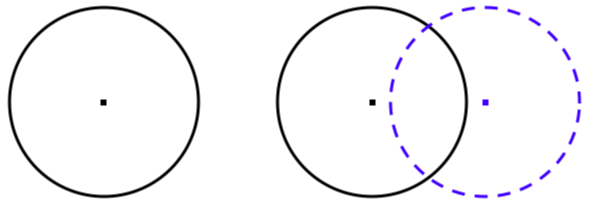
\includegraphics[scale=0.35]{./figures/snapped-to-ap-1}
		\caption{Availability zones of Message with k=0 (not snapped yet) to the left and k=1 (snapped to 1 Access Point) to the right}
	\end{figure}
	\vspace{1mm}
	\begin{figure}[h]
		\centering
		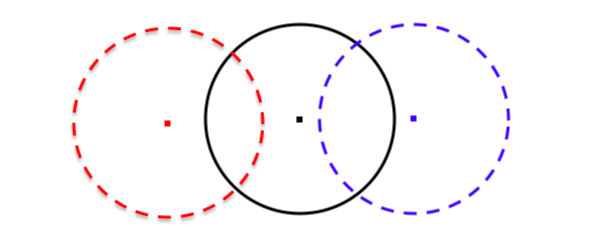
\includegraphics[scale=0.35]{./figures/snapped-to-ap-2}
		\caption{Availability zones of Message with k=2 (snapped to 2 Access Points)}
	\end{figure}
	\vspace{1mm}
	\begin{figure}[h!]
		\centering
		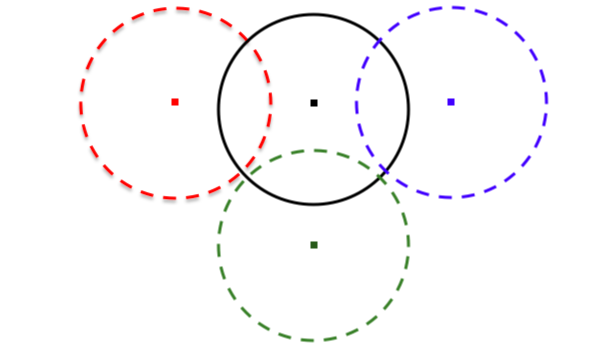
\includegraphics[scale=0.35]{./figures/snapped-to-ap-3}
		\caption{Availability zones of Message with k=3 (snapped to 3 Access Points)}
	\end{figure}
	\begin{figure}[h!]
		\centering
		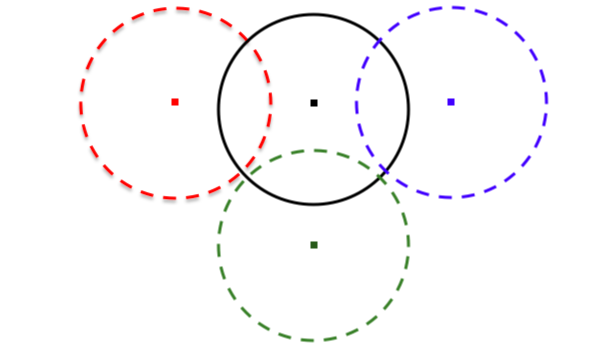
\includegraphics[scale=0.35]{./figures/snapped-to-ap-4}
		\caption{Special Case: Message with k=3 where there is no overlap between availability zones of the copies}
	\end{figure}

\newpage
\subsection{Implementation}
We will explain the implementation of this feature step by step below:
\begin{itemize}
	\item The very first point is to attach an \textit{originalAnchor} to the message (which is the point where the message was originally generated).
	\begin{lstlisting}[language=java]
	m.addProperty("originalAnchor", m.getProperty("anchor"));
	\end{lstlisting}
	\item The settings for the number of Access Points to snap to (\textit{kNextAPs}) is fetched inside \textit{FloatingContentRouter}.
	\begin{lstlisting}[language=java]
		if (fcSettings.contains(FC_NUM_OF_APS))
			kNextAPs = fcSettings.getInt(FC_NUM_OF_APS);
	\end{lstlisting}
	\item When message transfer is complete (\textit{messageTransferred} method in \textit{FloatingContentRouter}), we need to check f the message need to be snapped to any Access Point (by checking \textit{kNextAPs} property of the message).:
	\begin{itemize}
		\item If the host does not have a wifi interface, the control is returned back to the caller.
		\begin{lstlisting}[language=java]
			if(!(this.getHost() instanceof DTNHostWithWifi)
				return m;
			\end{lstlisting}
		\item If the receiving node is not an access point, the control is returned back to the caller.
		\begin{lstlisting}[language=java]
			DTNHostWithWifi receivingNode = (DTNHostWithWifi) this.getHost();
			if(receivingNode.getMode() != DTNHostWithWifi.AP)
				return m;
		\end{lstlisting}

		\item \textit{kNextAP} for the copied message is set to 0.
		\begin{lstlisting}[language=java]
			m.updateProperty(FC_NUM_OF_APS, 0);
		\end{lstlisting}

		\item The \textit{anchor} of the copy is set to the location of the access point if the message had been already anchored to this access point and the message still can be anchored to access points (\textit{kNextAPs>0}). Decrease \textit{kNextAPs} only if the message was not previously anchored to this access point.
		\begin{lstlisting}[language=java]
		if ((int) msg.getProperty(FC_NUM_OF_APS) > 0 || (anchorAccessPoints != null && anchorAccessPoints.contains(receivingNode.toString()))) {
			m.updateProperty(FC_ANCHOR, receivingNode.getLocation().clone());

			if((int) msg.getProperty(FC_NUM_OF_APS) > 0)
				msg.updateProperty(FC_NUM_OF_APS, (int) msg.getProperty(FC_NUM_OF_APS) - 1);
		}
		\end{lstlisting}
		\item The access point ID is added to the list of APS (\textit{anchorAPs}) property of the message. This helps us in re-snapping the message to the access point if the access points get a new copy of the same message.
		\begin{lstlisting}[language=java]
		anchorAccessPoints.add(receivingNode.toString());
		msg.updateProperty(FC_ANCHOR_APS, anchorAccessPoints);
		m.updateProperty(FC_ANCHOR_APS, anchorAccessPoints);
		\end{lstlisting}
		\item The access point location is added to the list of APS (\textit{anchorAPsLocation}) property of the message. This is used to make sure that the new availability zones are also accounted for before trying to delete a message.
		\begin{lstlisting}[language=java]
		anchorAccessPointsLocations.add(receivingNode.getLocation().clone());
		msg.updateProperty(FC_ANCHOR_APS_LOC, anchorAccessPointsLocations);
		m.updateProperty(FC_ANCHOR_APS_LOC, anchorAccessPointsLocations);
		\end{lstlisting}
	\end{itemize}
\end{itemize}
\subsubsection{Changes to Message Deletion Algorithm}
Here we are making sure that the message is deleted only after it is outside of the new availability zones (in case a message is snapped to access point, we need to check that the message is outside all the availability zones for that message).
\begin{lstlisting}[language=java]
for (Message m : m_set) {
	ArrayList<Coord> locations;
	try {
		locations = new ArrayList<Coord>((HashSet<Coord>)m.getProperty(FloatingContentRouter.FC_ANCHOR_APS_LOC));
	} catch(NullPointerException ignored) {
		locations = new ArrayList<>();
	}

	locations.add(0, (Coord)m.getProperty(FC_ANCHOR));
	locations.add(1,(Coord)m.getProperty(FC_ANCHOR_ORIGINAL));

	int counter = 0;
	while(counter<locations.size()) {
		distance_curr = loc.distance(locations.get(counter));
		if ((deletion_check(distance_curr, (Double) m.getProperty(FC_R), (Double) m.getProperty(FC_A)) != 1))
				break;
		counter ++;
	}
	if(counter == locations.size() && !d_list.contains(m.getId()))
		d_list.add(m.getId());
}
\end{lstlisting}
\subsection{Configuration}
\begin{lstlisting}[language=bash]
FloatingContentRouter.kNextAPs = 1
\end{lstlisting}
In the above listing, we are setting the number of access points a message can snap to 1. It means that each message can snap to 1 access points at maximum.
\newpage
\section{Access Points Data}
\subsection{Concept}
\subsubsection{Data Collection}
We are using the access points database from RadioCells \cite{wifi-data}. The database has a number of tables, however, we are only concerned with \textit{wifi\_zone}. We are only using \textit{latitude} and \textit{longitude} data.
\subsubsection{Data Processing}
We follow the following steps to process the data for the ONE Simulator:
\begin{enumerate}
	\item The data from access points database (which is a SQLite database) \cite{wifi-data} is exported to a text file.
	\item The data is processed by removing the double quotes and separating latitude and longitude by a comma (,).
	\item To make sure that the coordinates are converted to the correct scaling, we add the boundary coordinates to the file. Below are the boundary coordinates:
	\begin{itemize}
		\item minimumLatitude,0
		\item maximumLatitude,0
		\item 0,minimumLongitude
		\item 0,maximumLongitude
	\end{itemize}
	\item The processed file is then passed to a Coordinate Converter which returns a WKT file with the transformed coordinates.
	\item The WKT file can then be used for setting up the access points on the map using \textit{StationaryMapBasedMovement}.
\end{enumerate}
\begin{figure}[h]
	\centering
	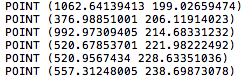
\includegraphics{./figures/access-points-data}
	\caption{Transformed Access Points Data}
\end{figure}
\subsection{Implementation}
A majority of the implementation is taken from Osm2Wkt \cite{mayer2010osm}. The implementation is pretty straight-forward. At first, we open the file and read the content into an array of Landmarks. \textit{Landmark} is a class that stores the original coordinate (represented by \textit{latitude} and \textit{longitude}) as well as the transformed coordinates (represented by \textit{x} and \textit{y}). The following code shows how the coordinates are stored as landmarks.
\begin{lstlisting}[language=java]
Scanner in = new Scanner(new FileReader(filePath));

while(in.hasNextLine()) {
	String text = in.nextLine().trim();
	if(text.length() > 0) {
		String[] coordinates = text.split(",");
		Landmark landmark = new Landmark(Double.parseDouble(coordinates[0]), Double.parseDouble(coordinates[1]));
		landmarks.add(landmark);
	}
}
in.close();
\end{lstlisting}
\vspace{2mm}
The coordinates are then transformed using \textit{transformCoordinates} \cite{mayer2010osm}. Finally, the coordinates are written in a WKT file which can be used by the ONE Simulator.\newline

To read the WKT file in ONE simulator, we have implemented \textit{StationaryMapBasedMovement} and \textit{MapNodeExtended} classes. The following table explains the functionality of each of these classes.

	\begin{center}
	    \begin{tabular}{ | l | p{8.8cm} |}
    		\hline
    		\textbf{Class} & \textbf{Details} \\ \hline
    		\textit{MapNodeExtended} & Inherits from the \textit{MapNode} class. It reads the WKT file and apply transformations (mirror and translation) to the location points. \\ \hline
    		\textit{StationaryMapBasedMovement} & Inherits from \textit{MapBasedMovement} class. Gets the list of transformed locations (from the WKT file) by passing it to \textit{MapNodeExtended}. \\ \hline
    	\end{tabular}
    	\captionof{table}{ONE Simulator: Classes for WKT based Node positioning} \label{tab:wktMapFiles}

	\end{center}
\newpage
Below code snippet shows the main functionality from \textit{StationaryMapBasedMovement}.
\vspace{3mm}
\begin{lstlisting}[language=java]
	public StationaryMapBasedMovement(Settings settings) {
		super(settings);

		String fileName = settings.getSetting(ROUTE_FILE_S);
		allNodes = MapNodeExtended.readNodes(fileName, getMap());
	}
	@Override
	public Coord getInitialLocation() {
		counter = (counter + 1) % allNodes.size();
		this.lastMapNode = allNodes.get(counter);
		return lastMapNode.getLocation();
	}
\end{lstlisting}
\label{lstlisting:node-positioning}
\captionof{lstlisting}{Main features of \textit{StationaryMapBasedMovement} class}

\vspace{10mm}
Below is the main code snippet from \textit{MapNodeExtended} class.
\vspace{3mm}
\begin{lstlisting}[language=java]
		WKTReader reader = new WKTReader();
		List<Coord> coords;
		File routeFile = null;

		//1.
		double xOffset = map.getOffset().getX();
		double yOffset = map.getOffset().getY();

		//2.
		List<MapNode> nodes = new ArrayList<MapNode>();
		try {
			routeFile = new File(fileName);
			coords = reader.readPoints(routeFile);
		}
		catch (IOException ioe) {
			throw new SettingsError("Couldn't read MapRoute-data file " +
					fileName + 	" (cause: " + ioe.getMessage() + ")");
		}

		//3.
		for (Coord c : coords) {
			if(map.isMirrored())
				c.mirror();

			c.translate(xOffset, yOffset);

			MapNode node = map.getNodeByCoord(c);
			if (node == null) {
				node = new MapNode(c);
			}
			nodes.add(new MapNodeExtended(node));
		}

		return nodes;
\end{lstlisting}
\captionof{lstlisting}{Getting List of all MapNodes (taken from \textit{MapNodeExtended})}
\vspace{5mm}
The following listing explains the main features of the above code:
\begin{enumerate}
	\item Normally, the map will have an offset of 0 on both the x and y axes. However, we can configure a different offset for the map. In this step, we fetch the offset for the map. This is necessary as we need to apply the same offset to all the nodes.
	\item All the points from the map files are read and stored as a list of coordinates.
	\item Here we check if the map has been mirrored (flipped on the X coordinate) because we need to apply the same transformation to each node. The node is then translated (as per offset of the map) and then a node is created which can be used in the simulation.
\end{enumerate}
\subsection{Configuration}
\begin{lstlisting}[language=bash]
Group1.movementModel = StationaryMapBasedMovement
Group1.routeFile = data/path_to_wkt_file/file_name.wkt
\end{lstlisting}
The above listing shows how we can configure ONE simulator to use a WKT map file (containing access points). First, we need to  set the \textit{movementModel} of the group to \textit{StationaryMapBasedMovement}. Then, we specify the relative path to the map file using \textit{routeFile}.
